\section {Measurement Circuitry: Version 1}

\subsection {Overview}

This section will describe version 1 of the circuitry proposed to measure the parameters needed to analyze a capacitor. It will present analytical and empirical assessments of each circuit section where feasible and applicable.

\subsection {Protection}

This subsection will explain the protection circuitry used to isolate parts of the circuit from the high DC voltage in the event of a failure.

\subsection {DC Bias}

The DC Bias circuitry will provide a controlled DC voltage from 0 to 500V. This voltage will be used to provide a DC bias for AC measurements, and to allow for charge/discharge measurements. A Stanford Research Supply PS350, 500VDC power supply will be used to generate the voltage. This supply will be controlled either manually or via its 0-10VDC external control input. Table: \ref{srsCtrl_table}. 

\begin{table}[ht!]
\centering
\begin{tabular}{| l | l | }
\hline
Input Scale      & 0 to +10V for 0 to 5kV                          \\ \hline
Input Impedance  & 1 M$\Omega$                                     \\ \hline
Accuracy         & $\pm 0.2\%$ of full scale                       \\ \hline
Update Rate      & 15 Hz                                           \\ \hline
Output Slew Rate & \textless 0.3s for 0 to full scale (full load)  \\ \hline
\end{tabular}
\caption{SRS-PS350 Analog Control Characteristics \cite{srsManual}\cite{srsCatalog}}
\label{table:srsCtrl_table}
\end{table}


Actual measurements of the supply can be seen in Table: \ref{srsGain_table}. As the table indicates, the supply does not exhibit reasonable control below 20mV of control signal (10V output). <---Need to include a noise or stability table over input voltages.--->

\begin{table}[ht!]
    \begin{tabular}{|l|l|l|l|l|}
    \hline
    Voltage In (V) & Voltage Out (V) & Absolute Error & Percent Error \\ \hline
    .01            & 7               & 2              & 40\%          \\ \hline
    .02            & 11              & 1              & 10\%          \\ \hline
    .1             & 52              & 2              & 4\%           \\ \hline
    .2             & 101             & 1              & 1\%           \\ \hline
    1              & 505             & 2              & 0.4\%         \\ \hline
    \end{tabular}
    \caption{SRS PS350 actual measured gain}
    \label{srsGain_table}
\end{table}


The RMS and peak-to-peak ripple voltage for the same range of outputs are shown in Table: \ref{srsNoise_table}.

\begin{table}[ht!]
    \begin{tabular}{|l|l|l|}
    \hline
    Voltage Out (V) & RMS Ripple (V) & PP Ripple (V) \\ \hline
    10              & 0.008          &               \\ \hline
    50              & 0.010          &               \\ \hline
    100             & 0.015          &               \\ \hline
    500             & 0.066          &               \\ \hline
    \end{tabular}
    \caption{SRS Noise over Range of output values}
    \label{table:srsNoise_table}
\end{table}


\begin{table}[ht!]
\centering
\begin{tabular}{| l | l | }
\hline
Input Scale      & 0 to +10V for 0 to 5kV                          \\ \hline
Input Impedance  & 1 M$\Omega$                                     \\ \hline
Accuracy         & $\pm 0.2\%$ of full scale                       \\ \hline
Update Rate      & 15 Hz                                           \\ \hline
Output Slew Rate & \textless 0.3s for 0 to full scale (full load)  \\ \hline
\end{tabular}
\caption{SRS-PS350 Analog Control Characteristics \cite{srsManual}\cite{srsCatalog}}
\label{table:srsCtrl_table}
\end{table}


%Need to add references to part datasheets
The block diagram in Figure: \ref{srsCtrlBlock} and the circuit in Figure: \ref{srsCtrl} show the logic for programatically controlling the SRS supply. The AD7391, a 12-bit DAC, is used to generate the desired control voltage for the SRS supply. Using a 1.0V xxxxx, a precision external reference, the output of the DAC swings from 0-1V with a resolution of 244uV. This sets the SRS supply from 0-500V with a resolution of 122mV. These numbers are theoretical and will degrade from ideal due to the SRS's response to the control signal, the noise levels in the system, and various other factors, such as temperature.

The AD7391 has a buffered output with a $1k\Omega$ output drive capability (for this application). Since the SRS supply is rated at a $1M\Omega$ input impedance, the specs should allow the DAC to directly control the power supply. To be on the safe side, an in-line, optional buffer is added to the circuit.

The AD7391 is controlled via a SPI bus connected to a microcontroller. The speed of this interface is not important because the system will only every change the output value of the DAC in between tests, not while collecting data. The DAC also has a CLR input that forces the output to 0V. The $10k\Omega$ pull down resistor ensures that the output sets the SRS supply to 0V upon start up for safety reasons.

As an added safety precaution, the SRS supply has the ability to enter in a manual voltage and current limit. The voltage limit will be set by the user to the maximum voltage of the particular test at hand.

Error calculations:...

\begin{figure}
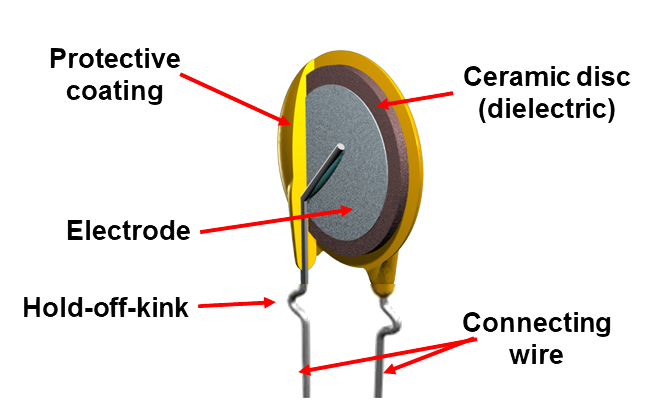
\includegraphics[keepaspectratio=true,scale=.5]{./figures/testImage.png}
\centering
%    \cite{capSite_df_vs_temp}
\caption{SRS Control Circuit Block Diagram}
\label{srsCtrlBlock}
\end{figure}


\subsubsection{Control Limiter}

This circuit section provides a set-point for the maximum allowed control signal to the SRS supply. It acts as a secondary safety limit. The primary limit being the SRS supply's front panel limit setting.

R802 and R805 provide a voltage divider; taking 5V down to 3V. R804 and R806 work with the potentiometer, R803, to provide a manual adjustment up to 3VDC. The diode in the feedback loop of U801 is known as a precision diode. \cite[ch5.1]{jungCook} It limits


List of things to explain:
\begin{enumerate}
    \item Super-diode
    \item resolution of DAC
    \item resolution of control
    \item effect of noise on the output
    \item logic for controlling the max control signal.
    \item overvoltage shunt?
    \item series resistor between last op amp and SRS
\end{enumerate}


\subsection {(Dis)Charge Circuitry}

This subsection will explain the circuit used to (dis)charge the DUT and the circuit used to measure the current through the DUT.

The basic purpose of this section is to measure the charge/discharge curves of the DUT by stepping the input voltage and then measuring the current through the device over time.

\begin{figure}[ht!]
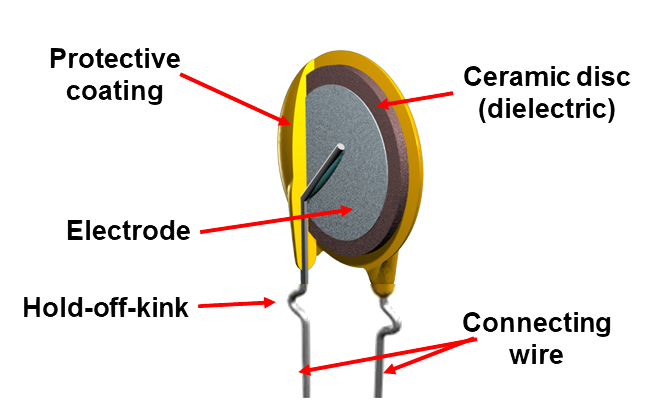
\includegraphics[keepaspectratio=true,scale=.5]{./figures/testImage.png}
\centering
\caption{(Dis)(Charge) Block Diagram}
\label{fig:cdlBlock}
\end{figure}


The block diagram depicted in Figure: \ref{cdlBlock} shows how this section will function. There are three basic modes:

Charging:
In this mode, the supply is set to the desired voltage and then stepped into the circuit with a relay. The input voltage sees a known resistor in series with the DUT to a virtual ground. The DUT will charge up to the input voltage according to its time constant. The virtual ground is made up of a transimpedance amplifier. It has the advantage of being able to measure on the low side of the DUT.

Discharging:
With the Charging side disconnected, a relay can connect the discharging circuitry to ground through a series resistor. The current measurement circuitry performs the same function, but with the opposite polarity measurement.

Leakage:
Once the DUT is charged to its full voltage, the steady state current can be measured over a much larger time period.

\subsubsection{Relay Control}
\begin{figure}
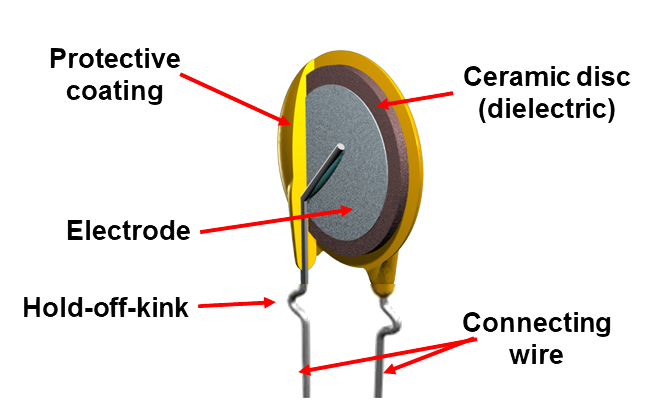
\includegraphics[keepaspectratio=true,scale=.5]{./figures/testImage.png}
\centering
%    \cite{capSite_df_vs_temp}
\caption{Relay Control Circuitry}
\label{cdlRelayCir_fig}
\end{figure}


Each relay is controlled with independent circuitry as shown in Figure: \ref{cdlRelayCir_fig}. The basic operation is that the input control signal (active high) switches either 5V or GND to the low side of the relay's coil. A ringback diode in series with a small valued resistor is in place to limit the coil's inductive spike while switching. Additionally there is a resistor + LED to indicate when an individual relay is active.

\subsubsection{Transimpedance Amplifier}
The transimpedance amplifier section is in place to provide a low side current measurement. It provides a 


\subsection {AC Signal Injection}

This subsection will cover the circuitry and supporting tech needed to inject an AC signal onto the DUT.

\subsection {Transformer}

This subsection describes the equations and operation of the transformer used to inject the AC signal ont the DUT.

\subsection {AC voltage Measurement}

This subsection describes the AC voltage amplitude and phase measurements. 

\subsection {Rise and Fall Times}

This subsection describes the circuitry used to mesaure the rise and fall times of the DUT.

